\section{Introduction}

\begin{frame}
	\frametitle{Definitions}
		The main objective of this chapter: \textbf{design} and \textbf{compensation} of single-input-sigle-output, linear, time-invariant control systems.
		\begin{itemize}
			\item Compensation: the modification of the system dynamics to satisfy the given specifications.
			\item Specifications (transient response and steady-state requirements): given before the design.
			\item Design by root-locus method: making a new root locus by adding poles and zeros to the system's open-loop transfer function.
			\item Compensator: another system inserted in parallel or in cascade with the system for the purpose of satisfying the specifications of the original system (e.g. lead, lag, lag-lead compensator's or PID controllers).
		\end{itemize}
\end{frame}

\begin{frame}
	\frametitle{Compensators}
	When a sinusoidal input is applied to the input of a network. We got a:
	\begin{itemize}
		\item lead network: if the steady-state output has a phase lead.
		\item lag network: if the steady-state output has a phase lag.
		\item lag-lead network: if we have phase lag and phase lead in the output but in different frequency regions (lag when the input has low frequency and lead in high frequency). 
	\end{itemize}
	$\rightarrow$ The amount of lag/lead is a function of the frequency. \vspace{4mm}
	
	A compensator with characteristic of a lead network, lag network, or lag-lead network is called a lead compensator, lag compensator, or lag-lead compensator. 
	
	\textbf{Remark}: with trial and error we find the optimal compensator
\end{frame}

\section{General design}

\begin{frame}
	\frametitle{Controllers}
		Sketching the problem:
		\begin{enumerate}
			\item We got a plant that not fulfil all the specifications (and we cannot change the parameters of the original system).
			\item We have to change other parameters such that the system will achieve all the specifications.
			\item These other parameters can be changed by changing the root locus of the closed-loop system. 
			\item So we look for a compensator that changes the root locus of the overall system such that the overall system achieve the specifications. 
			\item We let the original system interact (cascade or parallel) with the compensator.
		\end{enumerate}
		\vspace{3mm}
		
		\textbf{Remark}: we only discuss continuous time systems. 
\end{frame}

\begin{frame}
	\frametitle{Root locus approach}
	Looking at the transfer function $G(s)$, we can see that the closed-loop poles depend on the gain $K$. We can now plot the locus of all possible roots of the characteristic equation: 
		$$1 + KG(s) = 0 $$
	as $K$ varies from $0$ to $\infty$. This results in a graph which can help us in selecting the best value of $K$.\\
	\vspace{1em}
	Furthermore, by studying the effects of additional poles and zeros, we can determine the consequences of additional dynamics in the loop. 
	\vspace{2mm}
	
	In \textbf{general}: we want to have the root loci of the system on the good locations.
\end{frame}

\begin{frame}
	\frametitle{Addition of poles/zeros}
	\underline{Addition of poles}:\\
	\begin{itemize}
		\item Pulls the root locus to the right.
		\item Lowers the system's relative stability.
		\item Slows down the settling of the response.
	\end{itemize}
	\vspace{3mm}
	
	\underline{Addition of zeros}:
	\begin{itemize}
		\item Pulls the root locus to the left.
		\item Increases the system's relative stability.
		\item Speeds up the settling of the response.
		\item Speeds up the transient response.
		\item Increases the anticipation of the system. 
	\end{itemize}
\end{frame}

\section{Lead compensation}

\begin{frame}
	\frametitle{Lead compensators}
		There are 3 ways to make a \underline{lead compensator}:
		\begin{enumerate}
			\item Electronic networks using operational amplifiers.
			\item Electrical RC networks.
			\item Mechanical spring-dashpot systems.
		\end{enumerate}
		\vspace{3mm}
		
		When to use the \underline{root locus approach} for lead compensator's:\\
		$\rightarrow$ When the specifications are given in terms of time-domain quantities. Examples:
		\begin{itemize}
			\item damping ratio
			\item rise time
			\item settling time
			\item maximum overshoot
			\item undamped natural frequency
		\end{itemize}
\end{frame}

\begin{frame}
	\frametitle{Lead compensators}
	Steps to make a lead compensator (in cascade with the original system):
	\begin{enumerate}
		\item Determine the locations of the desired dominant poles (from the specifications).
		\item Draw the root locus of the uncompensated system. If we change the gain, then the poles will change. If we can achieve the locations of the desired poles on this way, then there is no need for a lead compensator. Else, if we cannot achieve the desired locations by adjusting the gain, then we have to make a lead compensator. 
		\item Assume the lead compensator with this transfer function: \\
		$C(s)=K_c \alpha\frac{Ts+1}{\alpha Ts+1}= K_c\frac{s+\frac{1}{T}}{s+\frac{1}{\alpha T}}$ with $0<\alpha<1$.
	\end{enumerate}
\end{frame}

\begin{frame}
	\frametitle{Lead compensators}
		\begin{enumerate}
			\setcounter{enumi}{3}
			\item Determining $\alpha$ and T:\\
			$\alpha$ and T are determined by the angle $\phi$. This is the angle $\angle(C(s))$ and must be equal to the difference between the angle of the desired pole and the angle of the original transfer function. \\
			Result: the closed-loop pole has the desired angle (angle of the desired pole). (And by determine T and $\alpha$ we determine the poles and zeros of the compensator.)
			\item Determine $K_c$ (=the open-loop gain) from the magnitude specifications.\\
			Result: the closed-loop pole has the desired magnitude. 
		\end{enumerate}
		\textbf{Remark}: if there is some freedom about the parameter $\alpha$, then take $\alpha$ as high as possible. 
\end{frame}

\begin{frame}
	\frametitle{Example 1: Lead compensators}
	\underline{Given}:
	\begin{itemize}
		\item Feed-forward transfer function: $G(s)=\frac{4}{s(s+2)}$
		\item Root locus plot of the uncompensated open-loop system:
		\begin{figure}
			\centering
			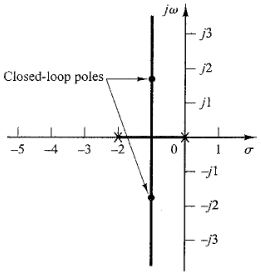
\includegraphics[width=0.3\linewidth]{Ex1_rootlocus}
		\end{figure}
	\end{itemize}
	\underline{Specifications}:
	\begin{itemize}
		\item Undamped frequency: $w_n=4$ rad/s
		\item Don't change the damping ratio
	\end{itemize}
\end{frame}

\begin{frame}
	\frametitle{Example 1: Lead compensators}
	\underline{Solution}:
	\begin{enumerate}
		\item Determine the desired poles: 
		\begin{itemize}
			\item The closed-loop transfer function: $\frac{C(s)}{R(s)}=\frac{4}{s^2+2s+4}$ with poles $s=-1\pm\sqrt{3}j$
			\item Damping ratio: $\zeta=0.5$
			\item Undamped natural frequency: 2 rad/s
			\item Static velocity constant: $K_v=2s^{-1}$
		\end{itemize}
		\vspace{3mm}
		$\begin{cases}
			\zeta \text{ must be the same} \rightarrow \text{let the angle of the poles constant}\\
			\text{Undamped frequency = 4rad/s} \rightarrow \text{magnitude of the poles}
		\end{cases}$
		\vspace{1mm}
		
		The desired poles are: $s=-2\pm j2\sqrt{3}$
		\vspace{3mm}
		
		\underline{Note}: in some cases, the desired poles can be obtained by adjustment of the gain. 
	\end{enumerate}
\end{frame}

\begin{frame}
	\frametitle{Example 1: Lead compensators}
	\underline{Solution}:
	\begin{enumerate}
		\setcounter{enumi}{1}
		\item  Find the sum of the angles at the desired location of one of the dominant closed-loop poles with the open-loop poles and zeros of the original system, and determine the necessary angle $\phi$ to be added so that the total sum of the angles is equal to $\pm 180^{\circ}(2k + 1)$. The lead compensator must contribute this angle $\phi$.\\
		Calculation of $\phi$: $$\angle(\frac{4}{s(s+2)})|_{s=-2+j2\sqrt{3}}=-210^{\circ}=-180^{\circ}-30^{\circ}$$
		And so we find $\phi=30^{\circ}$.
	\end{enumerate}
\end{frame}

\begin{frame}
	\frametitle{Example 1: Lead compensators}
	\underline{Solution}:
	\begin{enumerate}
		\setcounter{enumi}{2}
		\item Determine the pole and zero of the compensator (there are many possibilities): we use an algorithm to find the the pole and zero and to get an $\alpha$ as big as possible:
		\begin{figure}
			\centering
			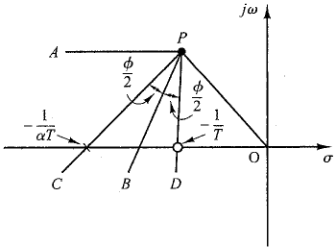
\includegraphics[width=0.6\linewidth]{Ex1_draw_algoritme}
		\end{figure}
	\end{enumerate}
\end{frame}

\begin{frame}
	\frametitle{Example 1: Lead compensators}
	\underline{Solution}:
	\underline{Algorithm} (figure previous slide):
	\begin{enumerate}
		\item Draw a horizontal line trough the desired dominant closed-loop pole P $\rightarrow$ PA
		\item Connect the origin with P $\rightarrow$ PO
		\item Bisect the two previous lines $\rightarrow$ PB
		\item Draw two lines that make an angle $\phi/2$ with the line PB $\rightarrow$ PC, PD
		\item The intersections of the negative real axis and the lines PC and PD are the zero and pole of the compensator. 
	\end{enumerate}
\end{frame}

\begin{frame}
	\frametitle{Example 1: Lead compensators}
	\underline{Solution}
	\begin{enumerate}
		\setcounter{enumi}{3}
		\item Transfer function of the lead compensator: $$C(s)=K_c\frac{s+\frac{1}{T}}{s+\frac{1}{\alpha T}} \text{ with } 0<\alpha<1$$
		(there are many solutions for T and $\alpha$). \\
		From the algorithm we get:\\ zero: -2.9 and pole: -5.4.\\
		$$T=\frac{1}{2.9}=0.345,\text{   } \alpha T=\frac{1}{5.4}=0.185$$
		So, we find $\alpha$: $\alpha=\frac{1}{5.4T}=0.537$.
	\end{enumerate}
\end{frame}

\begin{frame}
	\frametitle{Example 1: Lead compensators}
	\underline{Solution}:
	\begin{enumerate}
		\setcounter{enumi}{4}
		\item Determine $K_c$ from the magnitude condition: the open-loop transfer function of the compensated system becomes:\\
		$C(s)G(s)=K_c\frac{s+2.9}{s+5.4}\frac{4}{s(s+2)}=\frac{K(s+2.9)}{s(s+2)(s+5.4)}$ with K=$4K_c$.\vspace{3mm}
		
		The magnitude condition:
		$$|\frac{K(s+2.9)}{s(s+2)(s+5.4)}|_{s=-2+j2\sqrt{3}}=1 \Rightarrow K=18.7 \Rightarrow K_c=\frac{K}{4}=4.68$$
		And we get the transfer function of the lead compensator:
		$$C(s)=4.68\frac{s+2.9}{s+5.4}$$.
	\end{enumerate}
\end{frame}

\begin{frame}
	\frametitle{Example 1: Lead compensators}
	\underline{Solution}:
	\begin{figure}
		\centering
		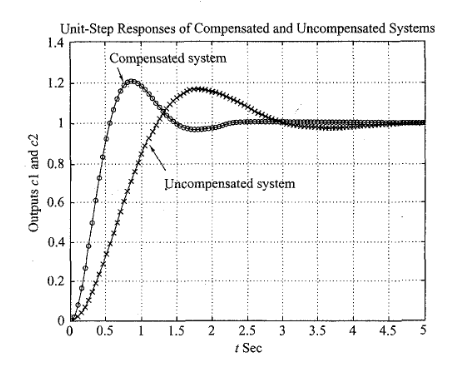
\includegraphics[width=0.7\linewidth]{Ex1_response}
	\end{figure}
\end{frame}


\section{Lag compensation}

\begin{frame}
	\frametitle{Lag compensators}
		 \textbf{Problem}: A system that satisfies the desired transient response but don't satisfy the steady-state. \\
		 $\rightarrow$ We have to compensate the system in such a way that it also satisfy the steady-state specifications (we have to make a lag compensator in cascade with the original system).
		 \vspace{4mm}
		  
		 \textbf{Concrete}:
		 \begin{itemize}
		 	\item Changing the steady-state by increasing the open-loop gain.
		 	\item Untouch the transient response by untouch the root locus in the neighbourhood of dominant closed-loop poles:
		 	\begin{description}
		 		\item [a)] poles and zeros close to each other;
		 		\item [b)] poles and zeros close to the origin;
		 		\item [c)] angle of the compensator must be small, $\angle(C(s))<5^{\circ}$.
		 	\end{description}
		 \end{itemize}
\end{frame}

\begin{frame}
	\frametitle{Lag compensators}
		$C(s)=K_c \beta\frac{Ts+1}{\beta Ts+1}= K_c\frac{s+\frac{1}{T}}{s+\frac{1}{\beta T}}$ with $\beta>1$\\
		\begin{itemize}
			\item Choose poles and zeros close together
			\item Choose $K_c$ close to 1 (if $K_c$ is exact 1, the transient response won't change)
			\item Take $\beta$ as large as possible
			\item Take T as large as possible 
		\end{itemize}
		\vspace{3mm}
		
		\textbf{Remark}: by the choice of $\beta$ and T, we have to take account of the reality (the physical realisation), so there is a limitation on the values.  \vspace{3mm}
		
		The \textbf{downside} of the lag compensator: the settling time will increase because the pole and zero of the closed-loop system are close to the origin. 
\end{frame}

\begin{frame}
	\frametitle{Steps to make a lag compensator}
		\begin{enumerate}
			\item Draw the root locus of the uncompensated open loop system and look for the dominant closed loop poles on the root-locus (from the specifications).
			\item The lag compensator is $C(s)=K_c \beta\frac{Ts+1}{\beta Ts+1}= K_c\frac{s+\frac{1}{T}}{s+\frac{1}{\beta T}}$.
			\item Calculate the static error constant $K_c$. 
			\item Calculate the new static error constant $K_c'$ if we achieve all the specifications.
			\item From this difference between $K_c$ and $K_c'$, we make the lag compensator. Now, we can determine $\beta$ and T. 
		\end{enumerate}
		\textbf{Remark}: we assume that the lag compensator achieved the transient response specifications. If not: make a lead-lag-compensator.
\end{frame}

\begin{frame}
	\frametitle{Steps to make a lag compensator}
		\begin{enumerate}
			\setcounter{enumi}{5}
			\item Draw the root locus of the compensated closed-loop system. Determine the locations of the dominant closed loop poles on the root-locus. 
			\item Adjust $K_c$ from the magnitude conditions such that the closed-loop poles lie at the desired location. ($K_c\approx 1$)
		\end{enumerate}
		\vspace{3mm}
		
		\underline{Some notes}:
		\begin{itemize}
			\item The ratio of the value of gain required in the specifications and the gain found in the uncompensated system is equal to the ratio between the distance of the zero from the origin and that of the pole from the origin.
			\item If the angle of the lag compensator is very small, then the original root loci and the new root loci are almost equal.
			\item Sometimes can be used both a lead or a lag compensator. 
		\end{itemize}
\end{frame}

\begin{frame}
	\frametitle{Example 2: Lag compensators}
	\underline{Given}:
	\begin{itemize}
		\item Feed-forward transfer function: $G(s)=\frac{1.06}{s(s+1)(s+2)}$
		\item Root locus plot of the uncompensated open-loop system:
		\begin{figure}
			\centering
			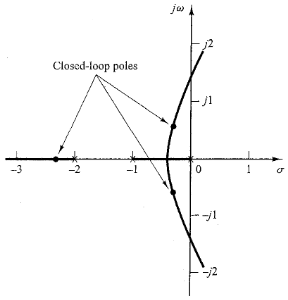
\includegraphics[width=0.3\linewidth]{Ex2_rootlocus}
		\end{figure}
	\end{itemize}
	\underline{Specifications}:
	\begin{itemize}
		\item Increase of the static velocity error constant $K_v$ to $5s^{-1}$
		\item Do not change the dominant closed-loop poles
	\end{itemize}
\end{frame}

\begin{frame}
	\frametitle{Example 2: Lag compensators}
	\underline{Solution}:
	\begin{enumerate}
		\item General calculations:
		\begin{itemize}
			\item The transfer function of the closed-loop system:
			$$\frac{Y(s)}{R(s)}=\frac{1.06}{s(s+1)(s+2)+1.06}$$ with poles: $s=-0.3307\pm j0.5864$
			\item Damping ratio: $\zeta=0.491$
			\item Undamped natural frequency: 0.673 rad/s
			\item Static velocity error constant: $K_v=0.53s^{-1}$
		\end{itemize}
	\end{enumerate}
\end{frame}

\begin{frame}
	\frametitle{Example 2: Lag compensators}
	\underline{Solution}:
	\begin{enumerate}
		\setcounter{enumi}{1}
		\item We assume a lag compensator C(s): $$C(s)=K_c\frac{s+\frac{1}{T}}{s+\frac{1}{T\beta}}$$
		\item To achieve the specifications: 
		\begin{itemize}
			\item $\beta\geq\frac{K^{desired}}{K^{current}}$ so we choose: $\beta=10$
			\item zero: s=-0.05 (from $\angle(C(s))<5^{\circ}$)
			\item pole: s=-0.005
		\end{itemize}
		\item C(s) becomes: 
		$$C(s)=K_c\frac{s+0.05}{s+0.005}$$
	\end{enumerate}
\end{frame}

\begin{frame}
	\frametitle{Example 2: Lag compensators}
	\underline{Solution}:
	\begin{enumerate}
		\setcounter{enumi}{4}
		\item Determine $K_c$:\\
		The open-loop transfer function of the compensated system becomes:\\
		$C(s)G(s)=K_c\frac{s+0.05}{s+0.005}\frac{1.06}{s(s+1)(s+2)} \Rightarrow K=1.06K_c$\\
		Holding the damping ratio the same, we find on the root locus plot (next slide) the poles: $s_{1,2}=-0.31\pm0.55j$.\\
		The open-loop gain is:
		$$K=|\frac{s(s+0.005)(s+1)(s+2)}{s+0.05}|_{s=-0.31+0.55j}=1.0235$$
		$\Rightarrow K_c=\frac{K}{1.06}=0.9656$
	\end{enumerate}
\end{frame}

\begin{frame}
	\frametitle{Example 2: Lag compensators}
	\underline{Solution}:
			\begin{figure}
				\centering
				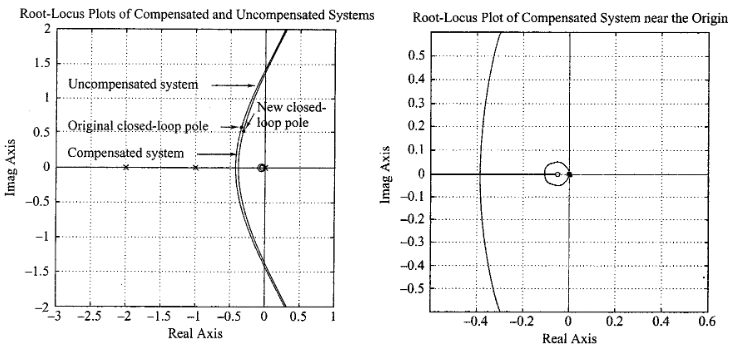
\includegraphics[width=1\linewidth]{Ex2_rootlocusnew}
			\end{figure}
\end{frame}

\begin{frame}
	\frametitle{Example 2: Lag compensators}
	\underline{Solution}:\\
	The transfer function of the lag compensator: 
	$$C(s)=0.9656\frac{s+0.05}{s+0.005}$$
	The transfer function of the compensated system:
	$$G(s)=\frac{1.0235(s+0.05)}{s(s+0.005)(s+1)(s+2)}$$
	The static velocity error constant:
	$$K_v=\lim_{s\to 0}sC(s)G(s)=5.12s^{-1}$$
\end{frame}

\begin{frame}
	\frametitle{Example 2: Lag compensators}
	\underline{Solution}:
	\begin{figure}
		\centering
		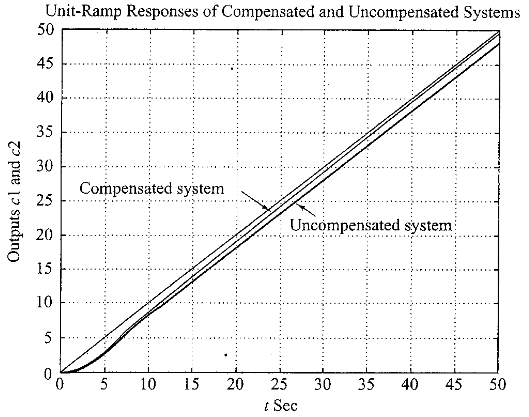
\includegraphics[width=0.65\linewidth]{Ex2_ramp}
	\end{figure}
\end{frame}

\begin{frame}
	\frametitle{Example 2: Lag compensators}
	\underline{Solution}:
	\begin{figure}
		\centering
		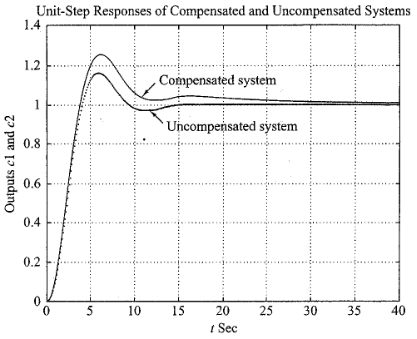
\includegraphics[width=0.65\linewidth]{Ex2_response}
	\end{figure}
\end{frame}

\begin{frame}
	\frametitle{Example 2: Lag compensators}
	\underline{Conclusions}:
	\begin{itemize}
		\item A pole and zero 
		$\begin{cases} \text{close to each other} \\ \text{close to the origin} \end{cases} \Rightarrow$ do not change the root-locus.
		\item The compensator increases the order of the system from 3 to 4 by adding a pole. 
		\item If a pole is further away from the j$\omega$ axis, the pole is less dominant and it will have less effect on the transient response.
		\item If the undamped natural frequency is low, then:
		\begin{itemize}
			\item the speed of the transient response will be less (the response will take a longer time to settle down);
			\item the overshoot of the step response will increase.
		\end{itemize}
	\end{itemize}
\end{frame}

\begin{frame}
	\frametitle{Resume}
	\underline{Effect}:
	\begin{itemize}
		\item Lead compensators increase the gain by high frequencies and so increases the bandwidth.
		\item Lag compensators reduce the bandwidth.
	\end{itemize}
	\underline{Advantages}:
	\begin{itemize}
		\item Lead compensators increase the dynamical response.
		\item Lag compensators reduce high frequency noise.
	\end{itemize}
	\underline{Disadvantages}:
	\begin{itemize}
		\item Lead compensators require extra gain and are sensitive to high frequencies (because the big bandwidth).
		\item Lag compensators worsens the transient response.  
	\end{itemize}
	\underline{Usage}:
	\begin{itemize}
		\item Lead compensators for quick transient response.
		\item Lag compensators for specified steady-state error.
	\end{itemize}
\end{frame}

\section{Lag-lead compensation}

\begin{frame}
	\frametitle{Lag-lead compensators}
		\underline{General}:\\
		Lead compensators: 
		\begin{itemize}
			\item speeds up the response;
			\item increase stability of the system.
		\end{itemize}
		Lag compensators:
		\begin{itemize}
			\item improves steady-state accuracy;
			\item reduces the speed of the response.
		\end{itemize}
		Lag-lead compensator:
		\begin{itemize}
			\item If both transient response and steady-state must be improved.
		\end{itemize}
		The lag-lead compensator has the advantages of both compensators. It has 2 poles and zeros, so the system has order 2.
\end{frame}

\begin{frame}
	\frametitle{Lag-lead compensators}
	The lag-lead compensator C(s) has this transfer function: 
	$$C(s)=K_c\frac{\beta (T_1s+1)(T_2s+1)}{\gamma (\frac{T_1}{\gamma}s+1)(\beta T_2s+1)}=
	K_c\left(\frac{s+\frac{1}{T_1}}{s+\frac{\gamma}{T_1}}\right)
	\left(\frac{s+\frac{1}{T_2}}{s+\frac{1}{\beta T_2}}\right)$$ with $\beta>1$ and $\gamma>1$.\vspace{4mm}
	
	Notes:
	\begin{itemize}
		\item The value $\beta T_2$ may not be too large, it must be physical realizable.
		\item  There are two cases of this type compensator: $\gamma\neq \beta$ and $\gamma= \beta$.
	\end{itemize}
\end{frame}

\begin{frame}
	\frametitle{Lag-lead compensators}
	Case 1:$\gamma\neq \beta$,  the design process is a combination of the design of the lead compensator and that of the lag compensator:
	\begin{enumerate}
		\item Determine the location of the closed-loop poles (from the specifications).
		\item The lead part of the compensator must contribute the angle $\phi$: $\phi=\angle$(desired pole)$-\angle$(uncompensated open-loop system).
		\item Calculate the parameters:
		\begin{itemize}
			\item Take $T_2$ as large as possible.
			\item Determine $T_1$ and $\gamma$ such that:\\ 
			$\angle(\frac{s_1+\frac{1}{T_1}}{s_1+\frac{\gamma}{T_1}})=\phi$
			\item Determine $K_c$ from the condition:\\
			$|K_c\frac{s_1+\frac{1}{T_1}}{s_1+\frac{\gamma}{T_1}}G(s)|=1$ with G(s) the open loop transfer function.
		\end{itemize}
	\end{enumerate}
\end{frame}

\begin{frame}
	\frametitle{Lag-lead compensators}
	Case 1:
	\begin{enumerate}
		\setcounter{enumi}{3}
		\item Determine $\beta$ if $K_v$ is given:
		$$K_v=\lim_{s\to0}sC(s)G(s)=\lim_{s\to 0}sK_c\left(\frac{s+\frac{1}{T_1}}{s+\frac{\gamma}{T_1}}\right)
		\left(\frac{s+\frac{1}{T_2}}{s+\frac{1}{\beta T_2}}\right)G(s)$$
		$$=\lim_{s\to0}sK_cG(s)\frac{\beta}{\gamma}$$
		\item Determine $T_2$ from:\\
		$$|\frac{s_1+\frac{1}{T_2}}{s_1+\frac{1}{\beta T_2}}|\approx 1 \text{ and } -5^{\circ}<\angle\left(\frac{s+\frac{1}{T_2}}{s_1+\frac{1}{\beta T_2}}\right)<0^{\circ}$$
	\end{enumerate}
\end{frame}

\begin{frame}
	\frametitle{Lag-lead compensators}
	Case 2: $\gamma= \beta$:
	\begin{enumerate}
		\item Determine the location of the closed-loop poles (from the specifications)
		\item If $K_v$ is specified, determine $K_c$ from:\\
		$$K_v=\lim_{s \to 0} sC(s)G(s)=\lim_{s\to 0}sK_c\left(\frac{s+\frac{1}{T_1}}{s+\frac{\beta}{T_1}}\right)
		\left(\frac{s+\frac{1}{T_2}}{s+\frac{1}{\beta T_2}}\right)G(s)$$
		$$=\lim_{s\to0}sK_cG(s)$$\item Determine the deficiency $\phi$, that must be contributed by the lead part of the lag-lead compensator, such that we get the dominant closed-loop poles on the desired location. 
	\end{enumerate}
\end{frame}

\begin{frame}
	\frametitle{Lag-lead compensators}
	Case 2: $\gamma= \beta$:
	\begin{enumerate}
		\setcounter{enumi}{3}
		\item Determine $T_1$ and$\beta$ from:
		$$|K_c\left(\frac{s+\frac{1}{T_2}}{s+\frac{1}{\beta T_2}}\right)G(s_1)|=1 \text{ and } \angle\left(\frac{s+\frac{1}{T_2}}{s+\frac{1}{\beta T_2}}\right)=\phi$$
		\item Determine $T_2$ from:\\
		$$|\frac{s_1+\frac{1}{T_2}}{s_1+\frac{1}{\beta T_2}}|\approx 1 \text{ and } -5^{\circ}<\angle\left(\frac{s+\frac{1}{T_2}}{s_1+\frac{1}{\beta T_2}}\right)<0^{\circ}$$
	\end{enumerate}
\end{frame}

\begin{frame}
	\frametitle{Example 3: Lag-lead compensators}
	\underline{Given}:
	\begin{itemize}
		\item Feed-forward transfer function: $$G(s)=\frac{4}{s(s+0.5)}$$
	\end{itemize}
	\underline{Specifications}:
	\begin{itemize}
		\item The damping ratio of the dominant closed-loop poles must be: $\zeta=0.5$
		\item Increase the undamped natural frequency to 5 rad/s
		\item Increase the static velocity error constant $K_v$ to 80 $s^{-1}$
	\end{itemize}
\end{frame}

\begin{frame}
	\frametitle{Example 3: Lag-lead compensators}
	\underline{Solution}:
	\begin{enumerate}
		\item General calculations:
		\begin{itemize}
			\item The closed loop poles: $s=-0.2500\pm1.9843j$
			\item Damping ratio: $\zeta=0.125$
			\item Undamped natural frequency: 2 rad/s
			\item Static velocity error constant: $K_v=8s^{-1}$
		\end{itemize}
	\item We use a lag-lead compensator with transfer function:
	$$C(s)=K_c\left(\frac{s+\frac{1}{T_1}}{s+\frac{\gamma}{T_1}}\right)\left(\frac{s+\frac{1}{T_2}}{s+\frac{1}{\beta T_2}}\right) \text{ with } \gamma>1, \beta>1, \gamma\neq\beta$$
	\end{enumerate}
\end{frame}

\begin{frame}
	\frametitle{Example 3: Lag-lead compensators}
	\underline{Solution}:
	\begin{enumerate}
		\setcounter{enumi}{2}
		\item The desired locations of the closed loop poles (from specifications) are: $s=-2.5\pm4.33j$
		\item Determine the angle of deficiency $\phi$:
		$$\angle\left(\frac{4}{s(s+0.5)}\right)|_{s=-2.5+4.33j}=-235^{\circ}=-180^{\circ}-55^{\circ} \Rightarrow \phi=55^{\circ}$$
		This angle must be contributed by the lead part of the compensator, such that the root locus passes through the desired closed-loop poles. 
	\end{enumerate}
\end{frame}

\begin{frame}
	\frametitle{Example 3: Lag-lead compensators}
	\underline{Solution}:
	\begin{enumerate}
		\setcounter{enumi}{4}
		\item Determine the zero and pole of the compensator (many possibilities):\\
		We take a zero at -0.5 (this will cancel the pole -0.5 of the plant) and a pole at -5.021 (such that the angle $\phi$ is contributed).
		The lead part becomes:
		$$K_c\frac{s+0.5}{s+5.021}$$
		and we find:
		\begin{itemize}
			\item $T_1=2$
			\item $\gamma=5.021/0.5=10.04$
			\item From the magnitude condition: \\
			$|K_c\frac{4(s+0.5)}{(s+5.021)s(s+0.5)}|_{s=-2.5+4.33j}=1 \Rightarrow K_c=6.26$
		\end{itemize}
	\end{enumerate}
\end{frame}

\begin{frame}
	\frametitle{Example 3: Lag-lead compensators}
	\underline{Solution}:
	\begin{enumerate}
		\setcounter{enumi}{5}
		\item Determine the lag part of the compensator:\\
		Determine $\beta$:
		$$K_v=\lim_{s \to 0}sC(s)G(s)=\lim_{s\to0}sK_c\frac{\beta}{\gamma}G(s)=4.988\beta=80 \Rightarrow \beta=16.04$$
		Determine $T_2$: $T_2$ must satisfy:
		$$|\frac{s+\frac{1}{T_2}}{s+\frac{1}{16.04T_2}}|_{s=s_1}\approx1 \text{ and } -5^{\circ}<\angle\left(\frac{s+\frac{1}{T_2}}{s+\frac{1}{16.04T_2}}\right)|_{s=s_1}<0^{\circ}$$\\
		 $\Rightarrow T_2=5$ with ($s_1=-2.5+4.33j$)
	\end{enumerate}
\end{frame}

\begin{frame}
	\frametitle{Example 3: Lag-lead compensators}
	\underline{Results}:\\
	\begin{figure}
		\centering
		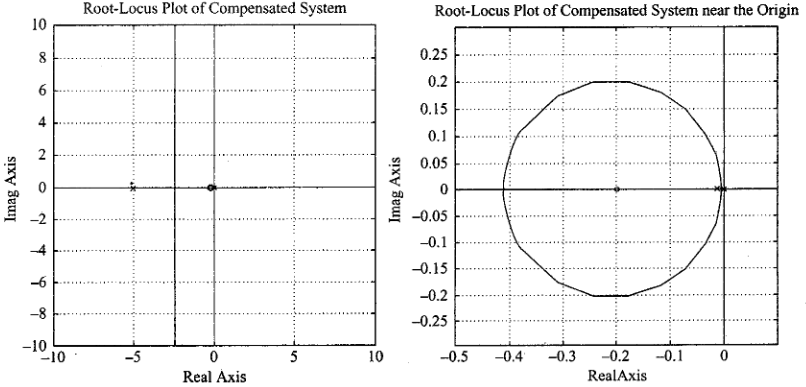
\includegraphics[width=1\linewidth]{Ex3_rootlocus}
	\end{figure}
\end{frame}

\begin{frame}
	\frametitle{Example 3: Lag-lead compensators}
	\underline{Results}:\\
	\begin{figure}
		\centering
		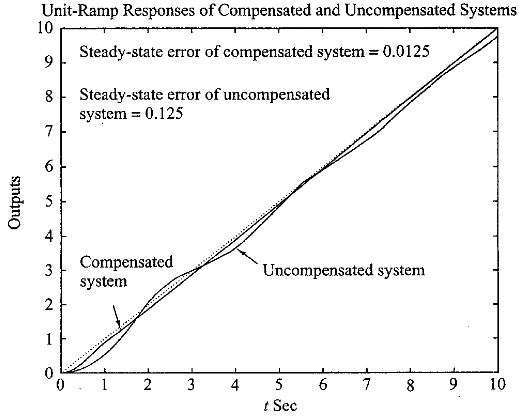
\includegraphics[width=0.65\linewidth]{Ex3_ramp}
	\end{figure}
\end{frame}

\begin{frame}
	\frametitle{Example 3: Lag-lead compensators}
	\underline{Results}:\\
	\begin{figure}
		\centering
		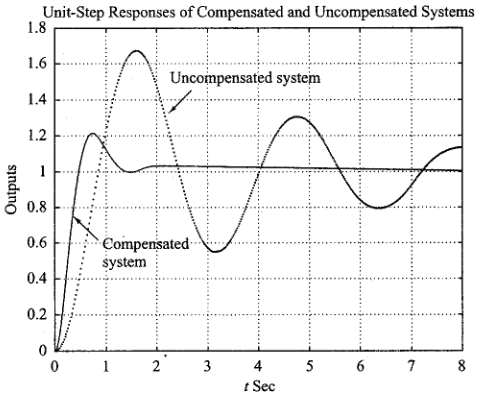
\includegraphics[width=0.65\linewidth]{Ex3_response}
	\end{figure}
\end{frame}

\begin{frame}
	\frametitle{Example 4: Lag-lead compensators}
	\underline{Given}:
	\begin{itemize}
		\item Feed-forward transfer function: $$G(s)=\frac{4}{s(s+0.5)}$$
	\end{itemize}
	\underline{Specifications}:
	\begin{itemize}
		\item The damping ratio of the dominant closed-loop poles must be: $\zeta=0.5$
		\item Increase the undamped natural frequency to 5 rad/s
		\item Increase the static velocity error constant $K_v$ to 80 $s^{-1}$
	\end{itemize}
\end{frame}

\begin{frame}
	\frametitle{Example 4: Lag-lead compensators}
	\underline{Solution}:
	\begin{enumerate}
		\item General calculations:
		\begin{itemize}
			\item The closed loop poles: $s=-0.2500\pm1.9843j$
			\item Damping ratio: $\zeta=0.125$
			\item Undamped natural frequency: 2 rad/s
			\item Static velocity error constant: $K_v=8s^{-1}$
		\end{itemize}
		\item We use a lag-lead compensator with transfer function ($\beta=\gamma$):
		$$C(s)=K_c\left(\frac{s+\frac{1}{T_1}}{s+\frac{\beta}{T_1}}\right)\left(\frac{s+\frac{1}{T_2}}{s+\frac{1}{\beta T_2}}\right) \text{ with } \beta>1$$
		\item The desired locations of the dominant closed-loop poles: $s=-2.5\pm 4.33j$
	\end{enumerate}
\end{frame}

\begin{frame}
	\frametitle{Example 4: Lag-lead compensators}
	\underline{Solution}:
	\begin{enumerate}
		\setcounter{enumi}{3}
		\item The compensated open-loop transfer function:
		$$C(s)G(s)=K_c \left(\frac{s+\frac{1}{T_1}}{s+\frac{\beta}{T_1}}\right)\left(\frac{s+\frac{1}{T_2}}{s+\frac{1}{\beta T_2}}\right)\frac{4}{s(s+0.5)}$$
		\item Calculation of the parameters:\\
		$K_v$ must be 80 $s^{-1}$:
		$$K_v=\lim_{s\to0}sG(s)C(s)=\lim_{s\to0}K_c\frac{4}{0.5}=8K_c=80 \Rightarrow K_c=10$$
	\end{enumerate}
\end{frame}

\begin{frame}
	\frametitle{Example 4: Lag-lead compensators}
	\underline{Solution}:
	\begin{enumerate}
		\setcounter{enumi}{4}
		\item From
		$$|\frac{s+\frac{1}{T_1}}{s+\frac{\beta}{T_1}}||\frac{40}{s(s+0.5)}|_{s=s_1}=1 \text{ and } \angle\left(\frac{s+\frac{1}{T_1}}{s+\frac{\beta}{T_1}}\right)|_{s=s_1}=55^{\circ}(=\phi)$$
		with $s_1=-2.5\pm 4.33j$,
		we get: $T_1=0.420$ and $\beta=3.503$.\\
		For $T_2$ we may choose 10.
	\end{enumerate}
	\underline{Results}:\\
	The transfer function of the compensator:
	$$C(s)=10\frac{(s+2.38)(s+0.1)}{(s+8.34)(s+0.0285)}$$
\end{frame}

\begin{frame}
	\frametitle{Example 4: Lag-lead compensators}
	\underline{Results}:\\
	The transfer function of the compensated open-loop system:
	$$C(s)G(s)=\frac{40(s+2.38)(s+0.1)}{(s+8.34)(s+0.0285)s(s+0.5)}$$
	\begin{figure}
		\centering
		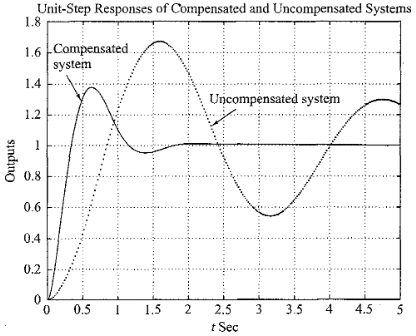
\includegraphics[width=0.48\linewidth]{Ex4_response}
	\end{figure}
\end{frame}

\begin{frame}
	\frametitle{Example 4: Lag-lead compensators}
	\underline{Results}:
	\begin{figure}
		\centering
		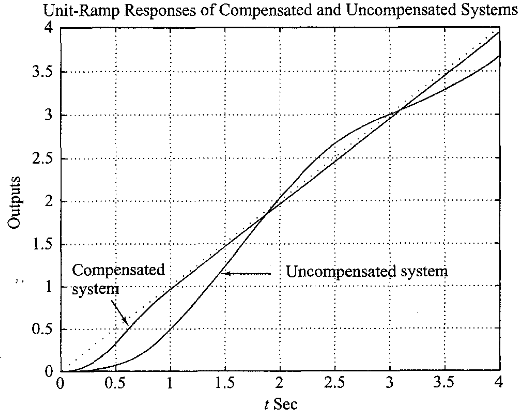
\includegraphics[width=0.7\linewidth]{Ex4_ramp}
	\end{figure}
\end{frame}

\section{Parallel compensation}

\begin{frame}
	\frametitle{Serial compensation}
	$\rightarrow$ Up to now, we have only discussed compensators in cascade with the system. \vspace{4mm}
	
	Derivation of the characteristic equation:\\
	\underline{Serial}:
	\begin{figure}
		\centering
		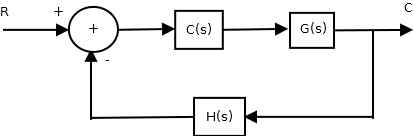
\includegraphics[width=0.7\linewidth]{Serial_compensator}
	\end{figure}
	The closed-loop transfer function: $\frac{C}{R}=\frac{GC}{1+GCH}$.\vspace{3mm}
	
	The characteristic equation is: $1+GCH=0$
\end{frame}

\begin{frame}
	\frametitle{Parallel compensation}
	Derivation of the characteristic equation:\\
	\underline{Parallel}:
	\begin{figure}
		\centering
		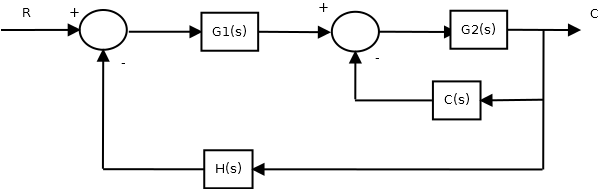
\includegraphics[width=0.9\linewidth]{Parallel_compensator}
	\end{figure}
	The closed-loop transfer function: $\frac{C}{R}=\frac{G_1G_2}{1+CG_2+G_1G_2H}$.\vspace{3mm}
	
	The characteristic equation is: $1+G_1G_2H+G_2C=0$
\end{frame}

\begin{frame}
	\frametitle{Parallel compensation}
	Derivation of the characteristic equation:\\
	\underline{Parallel}:\\
	If we divide the characteristic equation by $1+G_1G_2H$ we obtain: $$1+\frac{CG_2}{1+G_1G_2H}=0$$
	Now, we define: $G_f=\frac{G_2}{1+G_1G_2H}$.\\
	So, the characteristic equation becomes: $1+CG_f=0$\\
	$\rightarrow$ This has the same form as the serial characteristic equation. So, the same methods can be applied. 
	\vspace{2mm}
	
	Notes:
	\begin{itemize}
	\item A parallel compensator system is called a velocity feedback system.
	\item The compensator can be seen as a gain element.
	\end{itemize}
\end{frame}

